
\textbf{Notation and learning the concepts:} 
Assume $f^0: \mathcal{X} \rightarrow \mathcal{Y}$ is a pre-trained Blackbox predicting the output from the input image. Also, $\displaystyle f^0(.) =  h^0 \circ \Phi(.) $. Here, $ \Phi: \mathcal{X} \rightarrow R^l $ is the image embeddings and $ h^0: R^l \rightarrow \mathcal{Y}$ is the classifier, classifying the output $\mathcal{Y}$ using the embeddings, $\Phi$. Our approach is applicable for both datasets with and without human-interpretable concept annotations. For datasets with the concept annotation $\mathcal{C} \in \mathbb{R}^{N_c}$ ($N_c$ being the number of concepts per image $\mathcal{X}$), we learn $t: R^l \rightarrow\mathcal{C}$ to classify the concepts using the embeddings. Per this definition, $t$ outputs a scalar value $c$ representing a single concept for each input image. 
%We adopt the concept learning strategy in PosthocCBM (PCBM)~\cite{yuksekgonul2022post} for datasets without concept annotation. 
%Specifically, we leverage a set of image embeddings with the concept being present and absent. Next, we learn a linear SVM to construct the concept activation matrix~\cite{kim2017interpretability} as $\boldsymbol{Q} \in\mathbb{R}^{N_c \times l}$. 
Finally we estimate the concept value as $c = \frac{<\Phi(x), q^i>}{||q_i||_2^2}$ $ \in \mathbb{R}$ utilizing each row $\boldsymbol{q^i}$ of $\boldsymbol{Q}$. Thus, the complete tuple of $j^{th}$ sample is $\{x_j, y_j, c_j\}$, denoting the image, label, and learned concept vector, respectively.

\textbf{Method Overview:} 
Figure \ref{fig:Schematic} summarizes our approach. We iteratively carve out an interpretable model from the given Blackbox. Each iteration yields an interpretable model (the downward grey paths in Figure \ref{fig:Schematic}) and a residual (the straightforward black paths in Figure \ref{fig:Schematic}).
We start with the initial Blackbox $f^0$.
At iteration $k$, we distill the Blackbox from the previous iteration $f^{k-1}$ into a neuro-symbolic interpretable model, $\displaystyle g^{k}: \mathcal{C} \rightarrow \mathcal{Y}$. Our $g$ is flexible enough to be any interpretable models \eg logistic classifier~\cite{yuksekgonul2022post, koh2020concept, barbiero2022entropy}. The \emph{residual} $r^k =f^{k-1} - g^k$ emphasizes the portion of $f^{k-1}$ that $g^k$cannot explain. We then approximate $r^k$ with $f^{k} = h^k(\Phi(.))$. $f^k$ will be the Blackbox for the subsequent iterations and be explained by the respective interpretable model. 
% Due to computational reasons, we only finetune $h^{k}$ to optimize for $r^k$. 
A learnable gating mechanism, denoted by $\pi^k : \mathcal{C} \rightarrow \{0,1\}$ (shown as the \emph{selector} in figure \ref{fig:Schematic}) routes an input sample towards either $g^k$ or $r^k$.
% In order to learn $\pi^k$, we use simple backpropagation while learning $g^k$. A
The thickness of the lines in Figure \ref{fig:Schematic} represents the samples covered by the interpretable models (grey line) and the residuals (black line). 
% Our method is designed such that it leaves a little number of samples for the last residual blackbox.
With every iteration, the cumulative coverage of the interpretable models increases, but the residual decreases. We name our method \emph{route, interpret} and \emph{repeat}.

\subsection{Neuro-Symbolic Knowledge Distillation}
Knowledge distillation in our method involves 3 parts: (1) a series of trainable selectors ,\emph{routing} each sample through the interpretable models and the residual networks, (2) A sequence of learnable neuro-symbolic interpretable models, each providing FOL explanations to \emph {interpret} the Blackbox, and (3) \emph{repeating} with Residuals for the samples that cannot be explained with their interpretable counterparts. 
We detail each component below.

\begin{figure}[h]
% \vskip 0.2in
\centering
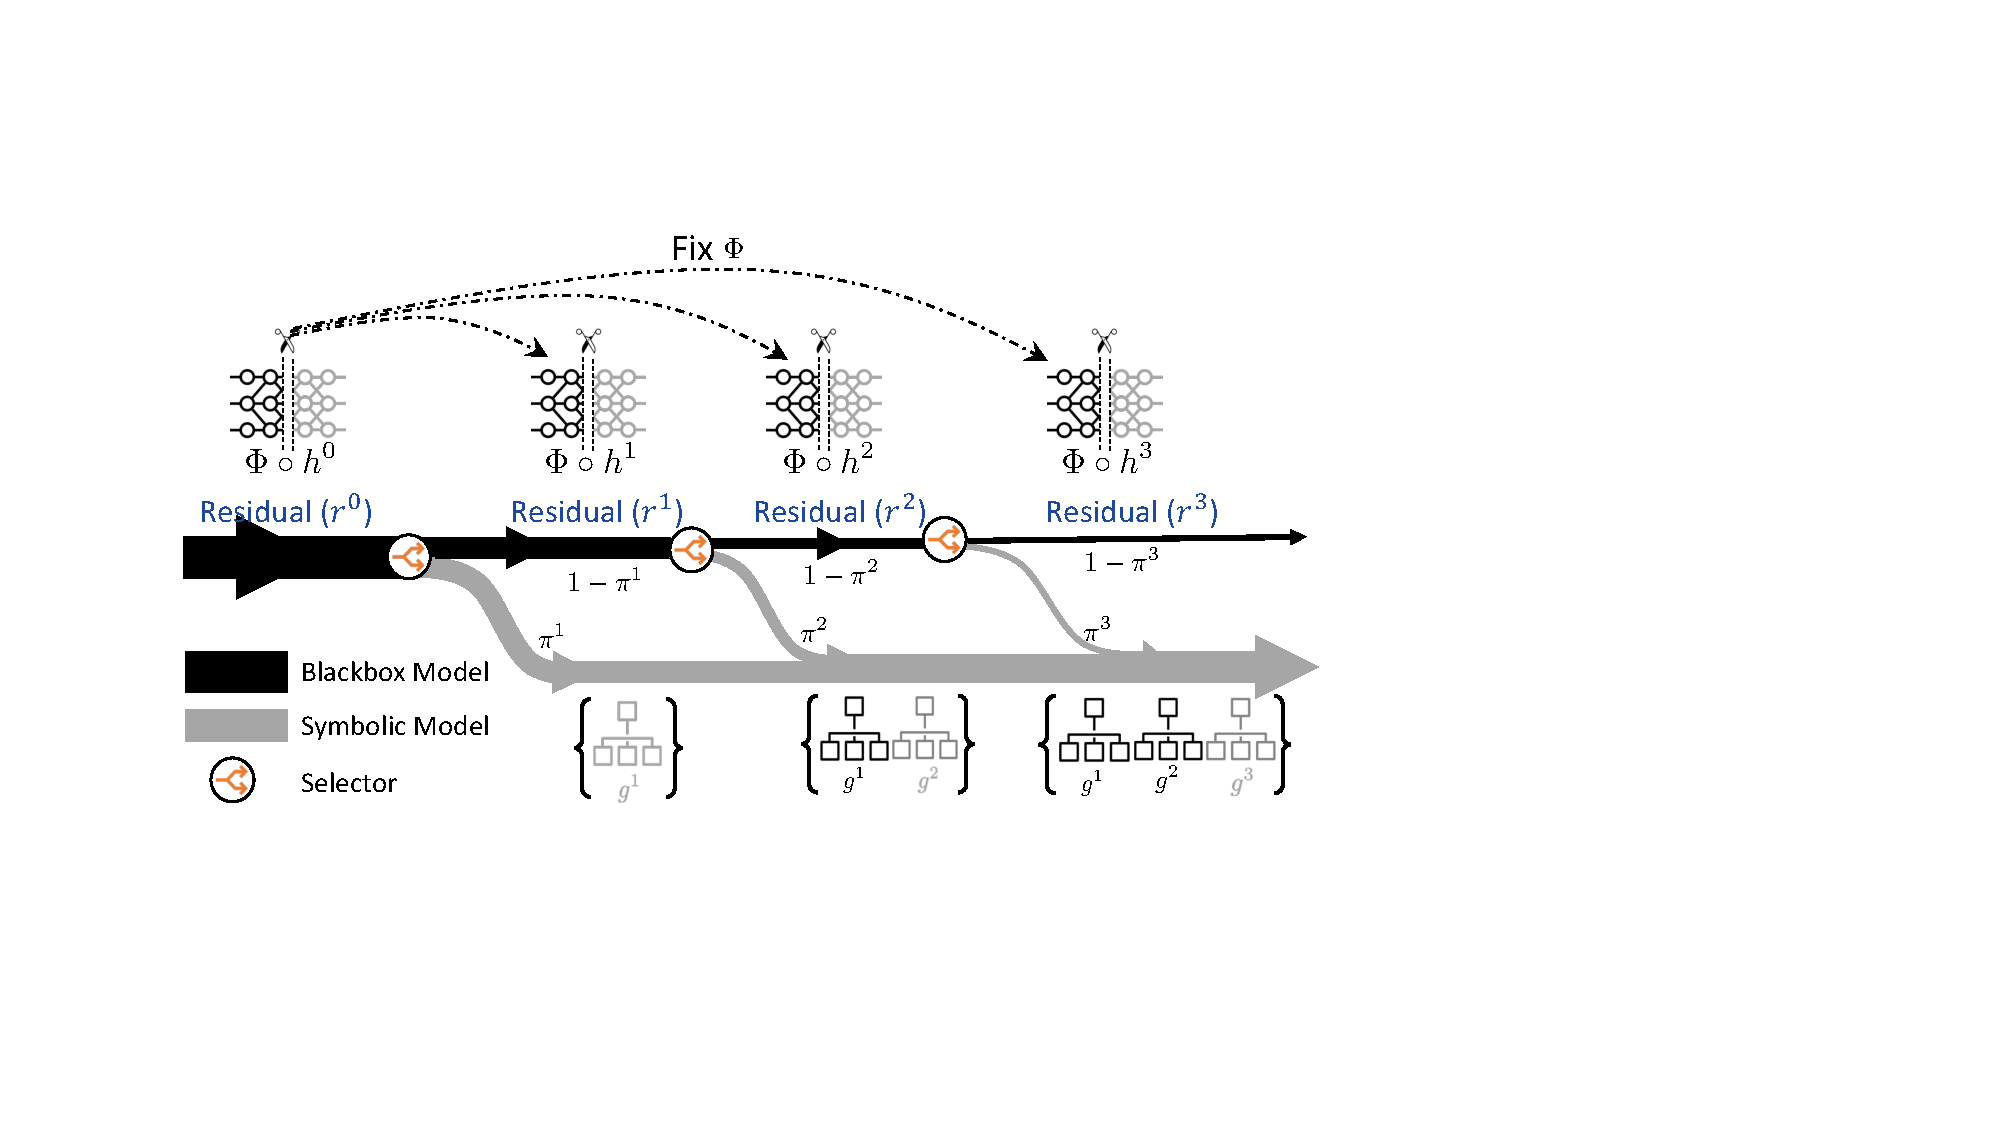
\includegraphics[width=\columnwidth]{figures/main/schematic.pdf}
\vskip -3pt
\caption{Schematic view of \emph{route, interpret} and \emph{repeat}. At iteration $k$, the selector \emph{routes} each sample either towards the interpretable model $g^k$ (to \emph{interpret}) with probability $\pi^k(.)$ or the residual $r^k = f^{k-1} - g^k$ with probability $1-\pi^k(.)$ (to \emph{repeat} in the further iterations). $f^{k-1}$ is the Blackbox of the $(k-1)^{th}$ iteration. $g^k$ generates FOL-based explanations for the samples it covers. Otherwise, the selector routes through the next step until it either goes through a subsequent interpretable model or reaches the last residual. Also, components in black and grey indicate the fixed and trainable modules in our model respectively. }
\label{fig:Schematic} 
\vskip -0.1in
\end{figure}

\subsubsection{The selector function}
As the first step of our method, the selector $\pi^k$ \emph{routes} the $j^{th}$ sample through the interpretable model $g^k$ or residual $r^k$ with probability $\displaystyle \pi^k(\boldsymbol{c_j})$ and $\displaystyle 1 - \pi^k(\boldsymbol{c_j})$ respectively, where $k$ $\in [0,K]$, with $K$ being the number of iterations.
We define the empirical coverage of the $\displaystyle k^{th}$ iteration as $\vspace{-0.08pt} \zeta(\pi^k) = \frac{1}{m}\sum_{j = 1} ^ m \pi^k(\boldsymbol{c_j}) \vspace{-0.081pt}$, the empirical mean of the samples selected by the selector for the associated interpretable model $\displaystyle g^k$, with $\displaystyle m$ being the total number of samples in the training set. Thus, the entire selective risk is:

\vskip -7.5pt
\begin{equation}
\label{equ: emp_risk}
\mathcal{R}^k(\displaystyle \pi^k, \displaystyle g^k) = \frac{\frac{1}{m}\sum_{j=1}^m\mathcal{L}_{(g^k, \pi^k)}^k\big(\boldsymbol{x_j}, \boldsymbol{c_j}\big)}{\zeta(\pi^k)} ,
\end{equation}
\vskip 2pt

where $\mathcal{L}_{(g^k, \pi^k)}^k$ is the optimization loss used to learn $\displaystyle g^k$ and $\displaystyle \pi^k$ together, discussed in section \ref{ns-optimization}. For a given coverage of $\displaystyle \tau^k \in (0, 1]$, we solve the following optimization problem:

\vskip -7.5pt
\begin{align}
\label{equ: optimization_g}
\theta_{s^k}^*, \theta_{g^k}^* = & \operatorname*{arg\,min}_{\theta_{s^k}, \theta_{g^k}} \mathcal{R}^k\Big(\pi^k(.; \theta_{s^k}), \displaystyle g^k(.; \theta_{g^k}) \Big) \nonumber \\ 
&\text{s.t.} ~~~ \zeta\big(\pi^k(.; \theta_{s^k})\big) \geq \tau^k,
\end{align}
\vskip 2pt

where $\theta_{s^k}^*, \theta_{g^k}^*$ are the optimal parameters at iteration $k$ for the selector $\pi^k$ and the interpretable model $g^k$ respectively. In this work, $\pi$s' of different iterations are neural networks with sigmoid activation. At inference time, the selector routes the $j^{th}$ sample with concept vector $\boldsymbol{c_j}$ to $\displaystyle g^k$ if and only if $\pi^k(\boldsymbol{c}_j)\geq 0.5$ for $k \in [0,K]$.

\subsubsection{Neuro-Symbolic interpretable models}
\label{ns-optimization}
In this stage, we design interpretable model $\displaystyle g^k$ of $k^{th}$ iteration  to \emph{interpret} the Blackbox $\displaystyle f^{k - 1}$ from the previous $(k-1)^{th}$ iteration by optimizing the following loss function:
\begin{equation}
\label{equ: g_k}
\resizebox{0.47\textwidth}{!}{$
\mathcal{L}_{(g^k, \pi^k)}^k\big(\boldsymbol{x_j}, \boldsymbol{c_j}\big) = \underbrace{\mystrut{2.6ex}\ell\Big(f^{k - 1}(\boldsymbol{x_j}), g^k(\boldsymbol{c_j})\Big)\pi^k(c_j) }_{\substack{\text{trainable component} \\ \text{for current iteration $k$}}}\underbrace{\prod_{i=1} ^{k - 1}\big(1 - \pi^i(\boldsymbol{c_j})\big)}_{\substack{\text{fixed component trained} \\ \text{in the previous iterations}}},
$}
\end{equation}

where the term $\pi^k(\boldsymbol{c_j})\prod_{i=1} ^{k - 1}\big(1 - \pi^i(\boldsymbol{c_j}) \big)$ denotes the probability of $j^{th}$ sample being routed through the interpretable model $g^k$. It is the probability of the sample going through the residuals for all the previous iterations from $0$ through $k-1$ (\ie $\prod_{i=1} ^{k - 1}\big(1 - \pi^i(\boldsymbol{c_j}) \big)$\big) times the probability of going through the interpretable model at iteration $k$ \big(\ie $\pi^k(\boldsymbol{c_j})$\big). 
Refer to Figure~\ref{fig:Schematic} for an illustration. We learn $\pi^1, \dots \pi^{k - 1}$ in the prior iterations and are not trainable at iteration $k$. As each interpretable model $g^k$ specializes in explaining a specific subset of samples (denoted by coverage $\tau$), we refer to it as an \emph{expert}. We use SelectiveNet's ~\cite{geifman2019selectivenet}  optimization method to optimize equation \ref{equ: optimization_g} since selectors need a rejection mechanism to route samples through residuals. Appendix \ref{app:loss} details the optimization procedure in equation \ref{equ: g_k}. We refer to the interpretable experts of all the iterations as a ``Mixture of Interpretable Experts'' (MoIE) cumulatively after training. Furthermore, we utilize Entropy-based linear layer neural network (ELL)~\cite{barbiero2022entropy} as the interpretable symbolic model $g$ to construct First Order Logic (FOL) explanations of a given prediction.

\subsubsection{The Residuals}
The last step is to \emph{repeat} with the residual $r^k$, as $\displaystyle r^k(\boldsymbol{x_j},\boldsymbol{c_j}) = f^{k - 1}(\boldsymbol{x_j}) - g^k(\boldsymbol{c_j})$.
We train $f^k = h^k\big(\Phi(.)\big)$ to approximate the residual $r^k$, creating a new Blackbox $f^k$ for the next iteration $(k+1$). This step is necessary to specialize $\displaystyle f^k$ over samples not covered by $g^k$. Optimizing the following loss function yields $\displaystyle f^k$ for the $\displaystyle k^{th}$ iteration:
\begin{equation}
\label{equ: residual}
\mathcal{L}_f^k(\boldsymbol{x_j}, \boldsymbol{c_j}) = \underbrace{\mystrut{2.6ex}\ell\big(r^k(\boldsymbol{x_j}, \boldsymbol{c_j}), f^k(\boldsymbol{x_j})\big)}_{\substack{\text{trainable component} \\ \text{for iteration $k$}}} \underbrace{\mystrut{2.6ex}\prod_{i=1} ^{k}\big(1 - \pi^i(\boldsymbol{c_j})\big)}_{\substack{\text{non-trainable component} \\ \text{for iteration $k$}}} 
\end{equation}

% \underbrace{\mystrut{2.6ex}\ell\big(f^{k - 1}(\boldsymbol{x_j}), g^k(\boldsymbol{c_j})\big)\pi^k(c_j) }_{\substack{\text{trainable component} \\ \text{from current iteration}}}
Notice that we fix the embedding $\displaystyle \Phi(.)$ for all the iterations. Due to computational overhead, we only finetune the last few layers of the Blackbox ($h^k$) to train $f^k$.
At the final iteration $K$, our method produces a MoIE and a Residual, explaining the interpretable and uninterpretable components of the initial Blackbox $f^0$, respectively. Appendix \ref{app:algo} describes the training procedure of our model, the extraction of FOL and the architecture of our model at inference.


\textbf{Selecting number of iterations $K$:} We follow two principles to select the number of iterations $K$ as a stopping criterion: 1) Each expert should have enough data to be trained reliably (
coverage $\zeta^k$). If an expert covers insufficient samples, we stop the process. 2) If the final residual ($r^K$) underperforms a threshold, it is not reliable to distill from the Blackbox. We stop the procedure to ensure the overall accuracy is maintained.